\documentclass[11pt]{article}
\usepackage[T1]{fontenc}
\usepackage[utf8]{inputenc}
\usepackage{lmodern,amsmath,amssymb,graphicx,geometry,microtype,setspace,booktabs,caption}
\usepackage[hidelinks]{hyperref}
\geometry{letterpaper,margin=1in}
\setlength{\parindent}{0pt}
\setlength{\parskip}{0.55em}
\setlength{\emergencystretch}{2em}
\captionsetup{labelfont=bf,font=small}
\renewcommand{\refname}{References}
\pagestyle{empty}
\renewcommand{\thefigure}{S\arabic{figure}}
\setcounter{figure}{1}
\begin{document}
\begin{figure}[!ht]\centering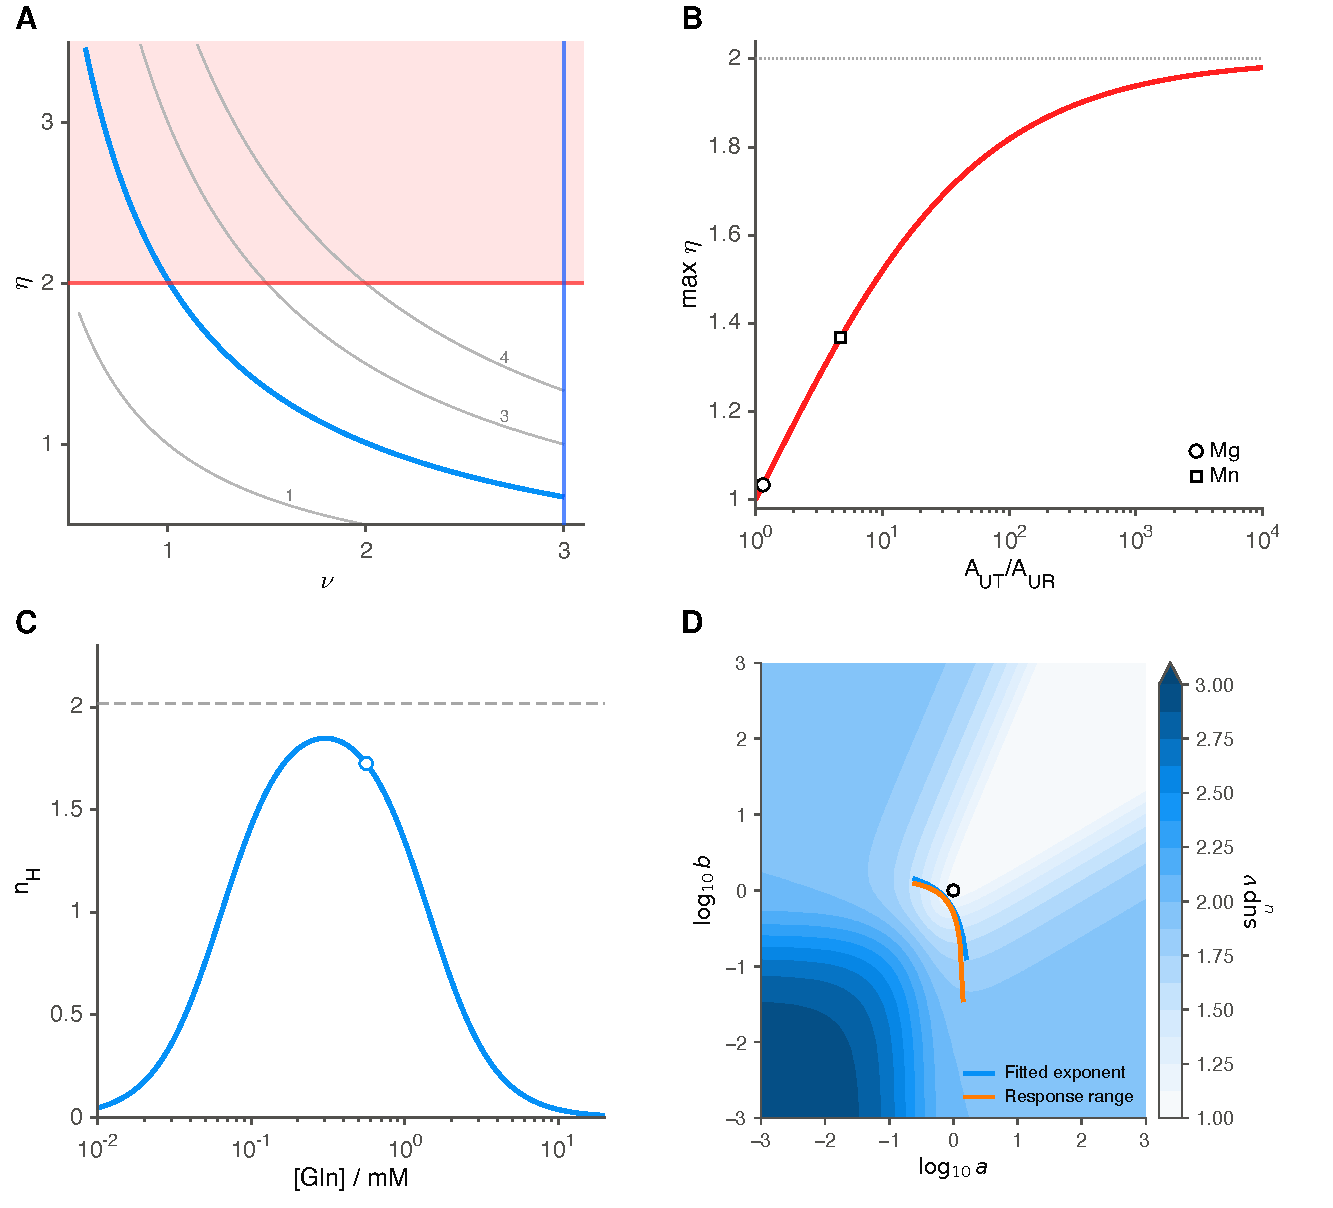
\includegraphics[width=\textwidth,height=0.60\textheight,keepaspectratio]{figure_inputs/FigS12_extended.pdf}\caption{\textbf{Local factorization and estimator-dependent ladder constraints.} (A) Gray contours denote local products nu eta of 1, 3, and 4. The blue contour is a numerical reference at 2.018, not a measured local sensitivity. Red marks eta=2, the ceiling of the specified reciprocal switch, and dark blue marks the trimer bound nu=3. (B) Maximum switch elasticity for the reciprocal switch in S2 Appendix, D7 when $A_{UT}$/$A_{UR}$ is at least one. Markers use the Mg and Mn kinetic-constant ratios discussed in the text. (C) Physical-occupancy local slope of the fitted first-layer curve, its fitted exponent of 2.018 (dashed), and midpoint local slope of 1.725 (circle). (D) Three-site ladder coefficients (1,3a,3b,1): distinct parameter loci reproduce coefficient ratio 1.11055 under fitted-exponent (blue) and response-range (orange) estimators. Color gives the maximum local ladder factor over input; the circle is the independent ladder. The loci are conditional calculations and show that the coefficient alone does not identify a unique ladder.}


\end{figure}
\end{document}
